After a comprehensive proposal for a cooperative perception system, including a novel modeling approach and an elaborate distributed software architecture, was presented in the previous chapters, this chapter aims to evaluate the system with respect to different aspects.

\Cref{sec:problem_analysis:goals_requirements} presented a set of goals and requirements to be met by the proposed system. While previous chapters already discussed how most of them are individually addressed, a few demand for further investigation or empirical assessment. Accordingly, a two-fold evaluation is conducted. The first part concerns with evaluating the proposed \textbf{software architecture} in terms of performance, specifically with respect to the requirements of scalability (NF-C2) and efficiency (NF-C3). The second part of the evaluation aims to assess the system's qualitative \textbf{performance in cooperative perception} tasks, motivated by the overall goal of this thesis to facilitate the improvement of connected, autonomous vehicles' average perception quality (cf. \cref{sec:problem_analysis:goals_requirements}). Both parts are split into four section each, that describe the respective evaluation's specific goal and methodology, explain certain implementation details, present the result and eventually discuss them in a brief conclusion.

\section{Performance Evaluation}
\label{sec:evaluation:performance_evaluation}
\Cref{sec:problem_analysis:goals_requirements} stated the non-functional requirements for the system to be able to handle 202 concurrent network participants at minimum and to aim for low latency and on-vehicle load. The following evaluation thoroughly assesses the previously developed system with respect to both criteria, i.e. \textbf{system scalability} and \textbf{communication efficiency}.

\subsection{Methodology}
\label{sec:evaluation:performance_evaluation:methodology}
First, one or more metrics need to be determined with respect to which the evaluation of the above criteria should be conducted.

Concerning scalability, a precise quantity is given as a requirement, which refers to the number of concurrent clients (i.e. vehicles, pedestrians, etc.) the system is expected to handle at minimum. Assuming a fixed per-vehicle message publish rate – which is in accordance with the previously introduced \textit{periodic push} principle – this translates to a \textbf{minimum number of observation messages}, i.e. state representations, the edge node must be able to process at a time. While the concrete message rate is a parameter that can be varied over the course of the evaluation, a hard minimum requirement of 202 concurrent vehicles is given. That is, assuming the entire system to operate at \SI{10}{Hz} (i.e. both client- and server-side publish rate), the fusion node must reliably process 2020 observations per second without dropping below that rate.

Concerning the second criterion, communication efficiency, average \textbf{latency in milliseconds} and average \textbf{message size in kilobytes} per vehicle and per observation are chosen to be used as metrics. In this specific context, latency refers to the average delay of a shared observation until received by an ego vehicle. While \cref{fig:communication_timeline} constitutes a detailed explanation of how this latency is composed, it essentially represents the average "'outdatedness"' of a CP message.

In order to gather these metrics, a minimalist sub-system of the entire CP software system is used. Accordingly, it still follows a client-server architecture with message broker and fusion node on one end and (simulated) ego vehicles on the other. Since we are only interested in quantitative measurements rather than in the messages' actual content, a newly created message generator program is used to artificially simulate observations instead of employing an actual Carla simulation with real Talky clients. Otherwise it would be infeasible to test with a large number of vehicles, due to exceedingly high computation load. The multi-threaded message generator is parameterized with (1) the target size of the generated occupancy grid observations, (2) the number of concurrent clients to simulate and (3) a per-client frequency at which to push messages to the backend. 

The test setup involves two physical machines, interconnected via a \SI{1}{\giga\bit\per\second} Ethernet network. One machine (AMD Ryzen 1600 \SI{3.2}{\giga\hertz} 6-core CPU, \SI{16}{\giga\byte} RAM, Ubuntu 18.04) runs the backend part of the system, i.e. message broker and edge node, while the message generator is run on the other (TODO).

\Cref{tab:performance_evaluation:constant_parameters} lists all fixed parameters used for the evaluation. Parameters marked with a star (*) are mentioned for completeness, but should not have any influence on the measured quantity. For the experiment, randomly generated occupancy grids within the same type 3 tile are used in the observation messages. Moreover, for performance measurements only an occupancy cell's state, but no information about its potential occupant (cf. \cref{subsec:concept_design:the_final_model}) is included, although the message size is measured for both cases in \cref{tab:performance_evaluation:message:sizes} for comparison. \Cref{tab:performance_evaluation:variable_parameters} lists all variable, evaluation-specific parameters to be tested in the evaluation in order to get insights about their respective impact on the final results. To test all combination of parameters, a grid search is conducted, i.e. a test is run for every combination in the Cartesian space of parameter values. 

\begin{table}
	\centering
	\begin{tabular}{|p{4.5cm}|p{2cm}|}
		\hline 
		\textbf{Parameter} & \textbf{Value} \\ \hline 
		\texttt{TILE\_1\_LEVEL} & \texttt{24} \\ \hline 
		\texttt{TILE\_2\_LEVEL} & \texttt{19} \\ \hline 
		\texttt{TILE\_3\_LEVEL} (*) & \texttt{15} \\ \hline 
		\texttt{MQTT\_QOS} & \texttt{1} \\ \hline 
		\texttt{DECAY\_FACTOR} (*) & \texttt{0}.11 \\ \hline 
		\texttt{OBSERVATION\_MAX\_AGE} & \texttt{3600} \\ \hline 
	\end{tabular}
	\caption[Performance Evaluation Constant Parameters]{Performance Evaluation Constant Parameters. See \cref{sec:implementation:configurable_parameters} for descriptions.}
	\label{tab:performance_evaluation:constant_parameters}
\end{table}

\begin{table}
	\centering
	\begin{tabular}{|p{3cm}|p{8.7cm}|p{3.5cm}|}
		\hline 
		\textbf{Paremeter} & \textbf{Description} & \textbf{Values} \\ 
		\hline 
		\texttt{N\_EGOS} & Numbers of concurrent simulated clients exchanging CP messages & \texttt{\{25, 50, 75, 100, 200, 400, 800, 1600\}} \\ 
		\hline 
		\texttt{RATE} & Frequency at which observations are periodically pushed by both server and clients (combines \texttt{FUSION\_RATE} and \texttt{OBSERVATION\_RATE}) parameters from \cref{sec:implementation:configurable_parameters} & \texttt{\{1, 5, 10\}} \\ 
		\hline 
		\texttt{GRID\_RADIUS} & Occupancy grid radius in number of cells. With $\lambda_1 = 24$ these are approx. equal to a grid size (i.e. observation range) of \texttt{\{52.8, 100.8\}} meters & \texttt{\{11, 21\}} \\ 
		\hline 
		\texttt{WITH\_OCCUPANT} & Whether or not to include occupant information for occupancy cells (effectively constant for measuring message rate and latency) & \texttt{\{false\}} \\ 
		\hline 
	\end{tabular}
	\caption{Performance Evaluation Variable Parameters}
	\label{tab:performance_evaluation:variable_parameters}
\end{table}

\begin{table}
	\centering
	\begin{tabular}{|p{6.2cm}|p{3.5cm}|p{3.5cm}|}
		\hline 
		& \texttt{GRID\_RADIUS = 11} & \texttt{GRID\_RADIUS = 21} \\ 
		\hline 
		\texttt{WITH\_OCCUPANT = true} & \SI{32}{\kilo\byte} & 1\SI{21}{\kilo\byte} \\ 
		\hline 
		\texttt{WITH\_OCCUPANT = false} & \SI{12}{\kilo\byte} & \SI{46}{\kilo\byte} \\ 
		\hline 
	\end{tabular}
	\caption[Evaluation Result: Average Observation Message Sizes]{Evaluation Result: Average Observation Message Sizes (occupied cells)}
	\label{tab:performance_evaluation:message:sizes}
\end{table}

\textbf{Message rate} and \textbf{message size} are measured at the fusion node. Therefor the code is extended in two places. First, code is added to track how often the \texttt{Publish()} method is called. Second, the sizes of all incoming messages are tracked and aggregated. \textbf{Latency} is measured at various places within fusion node and Talky client to get insights about how it is exactly composed. \Cref{fig:communication_timeline} illustrates all relevant steps within one round trip of cooperative perception that add delay to the total latency. The average durations $d_{i \in [0..6]}$ between these instants $t_{j \in [0..7]}$ are measured as part of this evaluation to help later optimization of certain system components and functions.

\begin{figure}
	\centering
	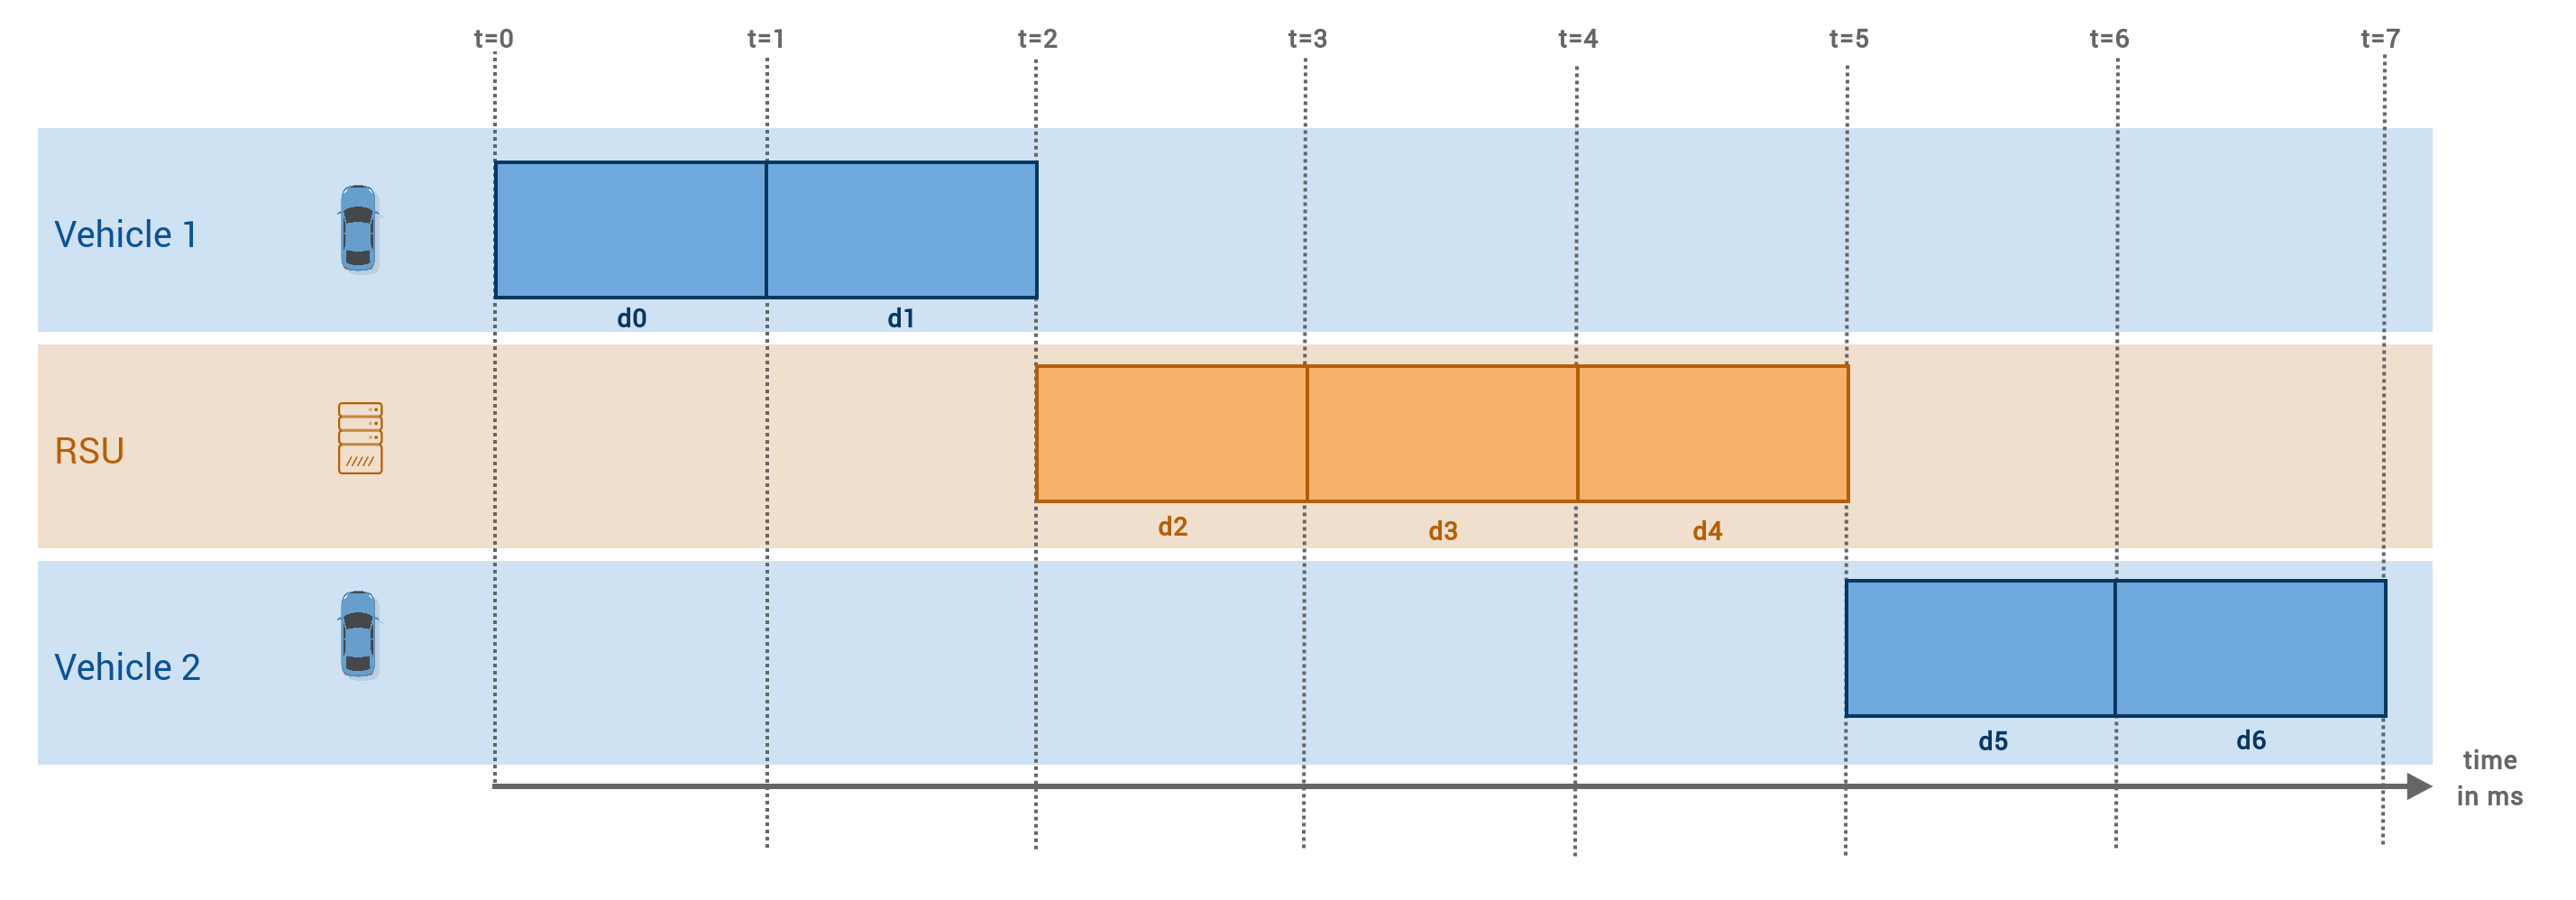
\includegraphics[width=1\linewidth]{98_images/communication_timeline}
	\caption{Timing Composition of Fusion Process}
	\label{fig:communication_timeline}
	\medskip
	\small
	\begin{enumerate}[t = 1:\ ]
		\item An observation is obtained by local sensory and low-level fusion (including ray casting-facilitated 5cell matching, etc., cf. \cref{subsec:implementation:talky_client}) \\
		\item The observation is encoded locally, i.e. represented as a PER model and serialized to Protobuf format
		\item The observation is received remotely, i.e. at the fusion node
		\item The observation is decoded remotely, i.e. deserialized from Protobuf and converted to process-local data structures
		\item The observation is remotely fused with other relevant observations from different observers, encoded to a PER model instance and serialized to Protobuf again
		\item The fused observation is received locally the ego vehicle
		\item The fused observation is decoded locally
	\end{enumerate}
\end{figure}
